\setNextFileName{LifeCycleOfACompiledMethod.html}
\begin{section}{Life Cycle of a Compiled Method}

In early implementations of Jikes RVM's adaptive system, compilation required holding a global lock that serialized compilation and also prevented classloading from occurring concurrently with compilation.  This bottleneck was removed in version 2.1.0 by switching to a finer-grained locking discipline to coordinate compilation, speculative optimization, and class loading. Since no published description of this locking protocol exists outside of the source code, we briefly summarize the life cycle of a compiled method here.

When Jikes RVM compiles a method, it creates a compiled method object to represent this particular compilation of the source method.  A compiled method has a unique id, and stores the compiled code and associated compiler meta-data. After a brief initialization phase, the compiled method transitions from uncompiled to compiling when compilation begins. During compilation, the optimizing compiler may perform speculative optimizations that can be invalidated by future class loading.  Each time the compiler so speculates, it records a relevant entry in an invalidation database.  Upon finishing compilation, the system checks to ensure that the current compilation has not already been  invalidated by concurrent classloading.  If it has not, then the system installs the compiled code, and subsequent  invocations will branch to the newly created code.

Each time a class is loaded, the system checks the invalidation database to identify the set of compiled methods to mark as obsolete,
because this classloading action invalidates speculative optimizations previously applied to that method.  A method may transition from either compiling or installed to obsolete due to a classloading-induced invalidation.  A method can also transition from installed to obsolete when the adaptive system selects a method for optimizing recompilation and a new compiled method is installed to replace it.

\begin{figure}
\centering
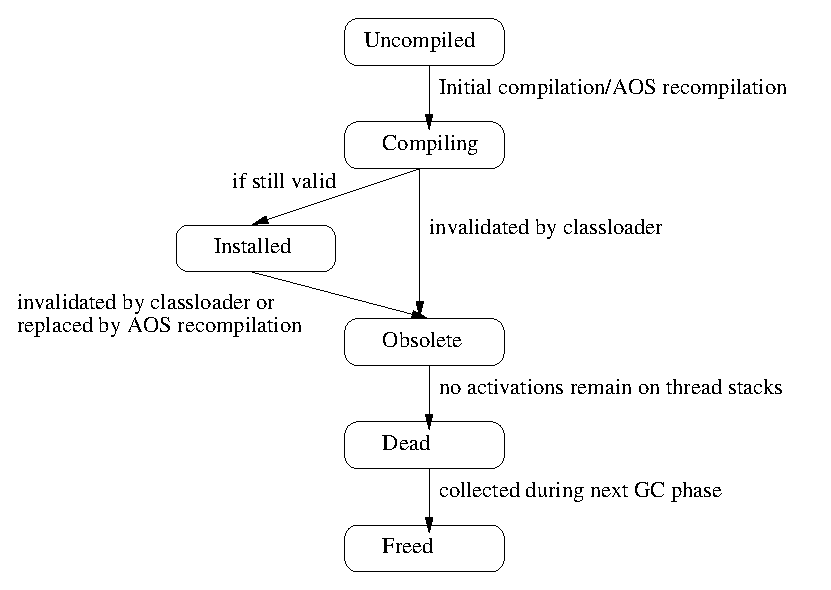
\includegraphics[width=\linewidth]{images/93224965.eps}
\caption{life cycle of a compiled method}
\end{figure}

Once a method is marked obsolete, it will never be invoked again.  However, before the generated code for the compiled method can be garbage collected, all existing invocations of the compiled method must be complete.  A compiled method transitions from obsolete to  dead when no invocations of it exist on any thread stack.  Jikes RVM detects this as part of the stack scanning phase of garbage collection; as stack frames are scanned, their compiled methods are marked as active.  Any obsolete method that is not marked as active when stack scanning completes is marked as dead and the reference to it is removed from the compiled method table.  It will then be freed during the next garbage collection.

\end{section}